%!TEX root = ../main.tex

\chapter{Introduction}
\markboth{Introduction}{}
%\vspace{-1.3in}

\paragraph{}
The Internet of Things refers to a relevantly new industry, which features the interconnection of every physical object with each other, using the internet as the bedrock for such a connection. In the era of Internet of Things, data is gathered from a myriad of sources in order to be processed and converted into wisdom, knowledge that will enables us to make smarter decisions in our everyday lives, in the planning of our cities and even in the damage control of natural disasters. Internet of Things is truly a frontier that will play a key role in the following years in a vast array of industries and domains.

\section{Reference Architecture}
The Internet of Things reference architecture, according to Cisco, can be summarised in Figure \ref{fig:iotarchsisco}, where there are 7 distinct layers of different activities that are conducted in a vertical slice of a typical Internet of Things system. The vertical slice refers to the fact that the system incorporates all 3 tiers of the systems (Constrained Devices or “Things", Edge, Cloud).  Throughout this thesis,  we will quote the various sensors, cameras, servos or even microcontrollers (like Arduino)  and other arbitrary \acrfull{iot} devices as “Constrained Devices”, in the sense that they have a very narrowly focused function and limited processing capability (if any).  While the typical architecture implies that layer 1 is at the “Things” tier, layers 2 and 3 at the Edge tier and layer 4 to 7 at the Cloud tier, the Edge computing paradigm pushes functionality from layer 4 to 7 down to layer 3.

\begin{figure}[h]
    \centering
    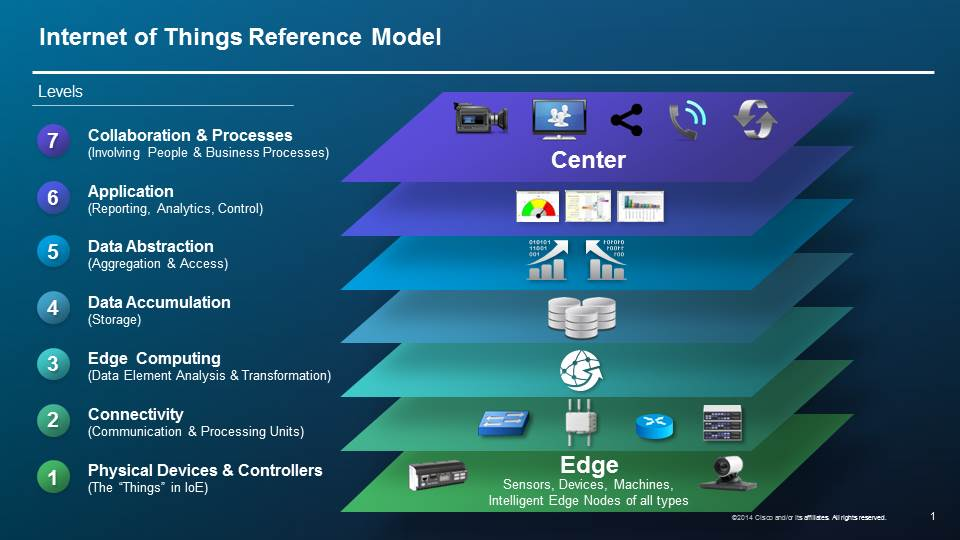
\includegraphics[width=\textwidth]{images/iotArchCisco.jpg}
    \caption{Illustration of the IoT Reference Model by Cisco\cite{iot-reference}}
    \label{fig:iotarchsisco}
\end{figure}

In terms of physical machines, a typical IoT hierarchical structure can be viewed in Figure \ref{fig:hier_arch_primer}, where the fog nodes communicate both with the cloud and with other fog nodes, either wirelessly or by wire.  Fog nodes can also function in a layered fashion, performing a different functionality according to their proximity to the data generators, which is still much closer than the cloud. Near the data source, fog nodes are mainly positioned in order to aggregate data, perform semantic notation and control the various actuators. Actuators are simply constrained devices that can interact with the physical world (e.g servos). Fog nodes that are upwards could perform more abstract functions, such as turning raw data into knowledge via processing. In this example, fog nodes can even be a non-homogenous group, even for the same stakeholder and system, as nodes closer to the source could be lighter in terms of processing and power consumption, such as the Raspberry pi \cite{rpi3}, while fog nodes that perform the bulk of pre-processing would be akin to a  \gls{microdc}(μDC).


\begin{figure}[h]
    \centering
    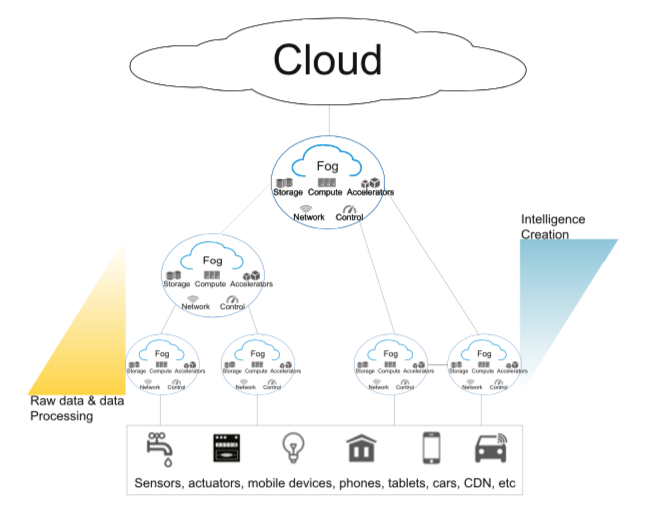
\includegraphics[width=\textwidth]{images/hierarchichal_architecture(from-primer).png}
    \caption{The hierarchical architecture of multiple fog computing layers\cite{ai2018edge} }
    \label{fig:hier_arch_primer}
\end{figure}

\section{Fog Computing}
The fog paradigm or more commonly known, \gls{edge-computing},  proposes that a part of the system’s intelligence and functionality must be implemented near the data source as opposed to the cloud-centric approach. While the terms“edge” and “fog” are commonly used interchangeably, the reader should be aware of the distinctions, especially when overviewing relevant bibliography. 

Edge computing refers to the concept of bringing resources closer to the data source, while fog computing was introduced by Cisco in 2014 as a terminology to define the edge computing as a standard\cite{linthicum2019}.  Edge computing has increased in popularity due to the fact that computational resources are becoming cheaper while the amount of data generated by devices is growing at an never before seen speed\cite{ericsson}. The placement of IoT resources with increasingly distributed architectures can be seen as akin to the evolution of the Internet, as at its beginnings, the mainframes were few and owned by trusted authorities (government, universities, etc.)\cite{leiner2009brief}. With the proliferation of the technology, we saw a democratization of the platform and an exponential increase in smaller servers with many different private stakeholders. 

The objective of the edge is to perform low-latency computation and some pre-processing on the raw data before sending them to the cloud. It offers a massive decrease of network costs since only a fraction of the data is actually transmitted to the cloud, offering at the same time, superior services to the consumers since the processing and decision making is happening near the source. These characteristics, can become even apparent, given the numbers of data throughput in modern applications. A boeing 787 generates about 5 GB of data per second, data that needs processing and which is highly sensitive, both in nature and decision making impact \cite{datafloq}. Another interesting example is an autonomous vehicle, which generate about 1GB of data \cite{finnegan2013}per second, data that need real time processing and decision making. This need for extreme low-latency can simply not be supported by a cloud solution, both in terms of network latency and scalability. We would need a cloud computing system that should be able to support effortlessly millions of cars (thus GB/s) while offering extreme low response time, something that at the moment is not technologically feasible.


\section{ The Edge computing paradigm in the Internet of Things}

On top of the above examples, if we narrow down the Edge Computing paradigm at the Internet of things, the case rests unchanged. Taking into consideration the increasing number of smart devices, such as smart-home (LED bulbs, speakers, home-automation, etc.) a cloud centric solution will not be able to cope with the amount of data \& processing needed, even if it is not as time critical as the examples above. A survey by Sony Ericsson indicates that by 2022 we could have 18 billion connected IoT devices\cite{ericsson}. 

Thus, the development of the IoT Edge Computing paradigm seems imperative in order to create the infrastructure needed to support this ecosystem. Figure \ref{fig:fog_comp_app} shows a sample of the many applications that exist for the Internet of things. The outermost layer of the image is populated by the constrained devices that have a specialised function over a a domain (e.g Power Supply), while the middle layer is populated of the Edge Nodes and finally, the innermost consists of the cloud that manages the inner layers and offers additional services (e.g long-term storage). It is interesting to comment that not only the number of distinct devices is reduced as we advance to the center of the cycle, but also, as we advance the homogeneity of the systems is increased. Constrained devices are highly specialized and thus numerous is numbers and in forms, while a datacenter can host all kinds of different applications, which of course share certain similarities (i.e they share certain elements, such as domain, stakeholder, critical factor).

In this thesis, we outline the architecture and main characteristics of an Internet of Things system that follows the Edge computing paradigm, with emphasis on data integrity and high availability. We will focus our architectural design \& implementation on the fog tier of the IoT stack, creating a layer that is agnostic both in terms of Constrained Devices and Cloud backend infrastructure. Our proposed architecture has the following key characteristics:
\begin{itemize}
 \item it is built on top of the microservices paradigm for extensive modularity and expandability
  \item it is based almost entirely on open source projects, so that we are able to contribute and showcase their incredible potential
 \item it exploits the unique characteristics of the container technology that is commonly used in cloud environments but modified for the needs and characteristics of the Edge.
 \item a novel blockchain based technology is used to store both the available application logic and data, in an effort to provide data integrity across the pipeline and facilitate  the high availability of the platform
\item the implementation is based on a Raspberry pi 3 micro-computer where we will attempt the dynamic handover of LoRa devices, between devices that belong to different stakeholders and have, perhaps, different functionality.
\end{itemize}

\begin{figure}[h]
    \centering
    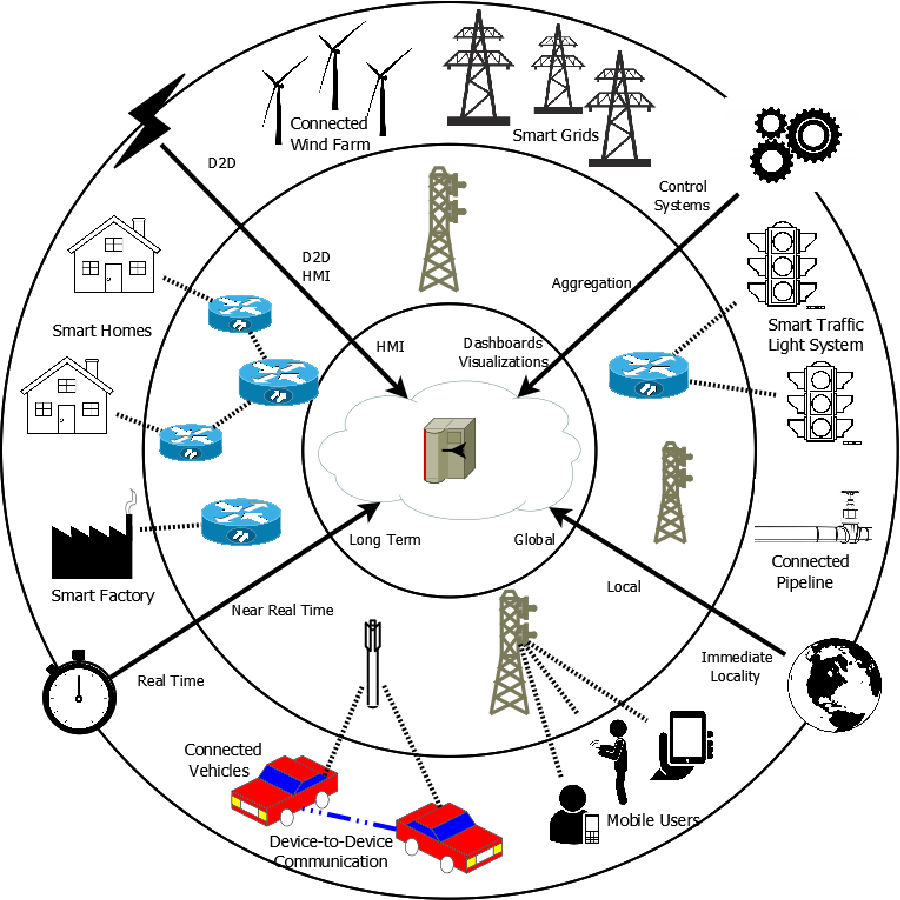
\includegraphics[width=0.7\textwidth]{images/fogComputingApplications(from-principles).png}
    \caption{The Internet of Things is relevant to an array of different domains\cite{dastjerdi2016fog}}
    \label{fig:fog_comp_app}
\end{figure}

Our proposed  Edge platform and prototype implementation, enables the Edge provider to dynamically execute applications and services demanded by clients,  “renting”, in essence, a part of their Edge Infrastructure to perform the application logic of a 3rd party. Enabling thus, the concept of \textbf{“IoT Edge computing as a Service”}, where the Edge Resources are actively offered and demanded in an IoT Edge Computing Marketplace. In this context, we outline a use-case in the domain of \gls{fault-tolerance}, where an Edge Node faces a critical failure and handovers its sensors and its services to another pre-determined Edge Node.

In Chapter \ref{ch:problem-statement} we underline the problem statement of this thesis and the state of art solutions that exist, in Chapter \ref{ch:system-architecture} we introduce the high level architecture while in Chapter \ref{ch:implementation} we give a proof of concept implementation in the form of a walkthrough tutorial. Finally in Chapter \ref{ch:discussion} there is a discussion on the various aspects of the implementation and our assumptions, in Chapter \ref{ch:results} we conclude with the results of this work and in Chapter \ref{ch:future-work} we talk about future work on this research vertical.
